\section{Computation and Fitting Procedures}\label{appFitting}

\textbf{
    In this section we provide more details on how we compute the VSFs and their scaling parameters.
    As described in Sect.~\ref{methods:vsf} the discussions in the main part of this manuscript are based on VSFs that are computed from average relative velocities. 
    This means the following:
}

\textbf{ 
    We map the 3D FLASH adaptive mesh refinement data of the original simulations \citepalias{IbanezMejia2016,IbanezMejia2017} onto uniform grid data cubes 40~pc on a side with 0.1~pc zones. 
%    Those cubes consist of 400$^3$ zones, each with a volume of (0.1~pc)$^3$, with the centres of the cubes being 
   centred on 
the centres of the molecular clouds. 
}

\textbf{
    The FLASH simulations take ten levels of resolution into account; and the decision which region is resolved up to which level depends on the density of the respective grid cell \citepalias{IbanezMejia2017}.
    Therefore, the original simulations cover a range of resolutions from 30.4~pc in regions of 
%mm $|$10$|$-- $|$20$|$~pc around the midplane of the modelled galactic plane
    with $|z| > 10$~kpc above and below the galactic midplane
down to 0.06--0.10~pc within (100~pc)$^3$ boxes around the centre of mass of the three molecular clouds presented in this manuscript, as well as in \citetalias{IbanezMejia2017} and \citetalias{Chira2018}. 
    Therefore, the resolution we have chosen for the data cubes corresponds to either the highest resolved level offered by the simulations
 (in the case of \texttt{M8}) or a slight
%mm ly lower resolved level
      coarsening of the most resolved level
(in the cases of \texttt{M3} and \texttt{M4}).
The zoom-in regions modelled at the highest resolution level extend well beyond the volume we 
%mm map into the box grid. 
      use in our analysis.
%mm
 We have adopted this size as it is sufficient for covering the clouds' volumes, and thus more efficient for further analyses. In addition, this choice protects us from resolution edge effects as the transitions from this resolution level to the next lowest are several tens of zones away. 
}

\textbf{
%mm    A consequence of mapping the data onto a regular box grid is that we can only offer a discrete representation of the velocity information. 
No matter whether a density threshold is applied or not, 
%mm this binning still represents an amount of data that is computationally hard to process.
     the 40 pc cubes still include too much data to compute complete velocity structure 
     functions including all lags from all points.
%mm For deriving and analysing
     Therefore, to derive
the VSFs we coarsen the grid of projected lag distances, $\ell_i = |\vec{\ell}|_i$
%mm , so that separates the range between 0.1 and 30~pc into 
    to cover the range 0.1--30~pc with
only 40 equidistant bins. 
}

\textbf{
    After mapping the data onto the 
%mm box grids 
     uniform grid,  
we apply two approaches: 
    The first considers only zones above the density threshold, $n_\mathrm{cloud}$.
%mm   This means that we pick only those cells from the data cubes that contain number densities equal to or larger than n$_\mathrm{cloud}$.
    These zones represent the starting points $\vec{x}$ (see Eqs.~\ref{equ:method:def_vsf}--\ref{equ:method:def_vsf_1d}).
    Our routine 
%mm goes to each of these cells and calculated the lag distance to
     calculates the lag distances between these zones and 
every other zone in the sample, as well as the relative velocities of the gas 
%mm that is simulated 
within the given zones. 
    The individual lag distances are 
%mm summarised into 
   binned using
spherical shells around the starting zones that range from inner radii $\ell_{i}$ to outer radii $\ell_{i+1}$. 
    By doing so, we compute the discrete VSFs presented in the main part of this paper with the relative velocities and product of densities, $\rho(\vec{x}) \cdot \rho(\vec{x}+\vec{\ell})$, measured from zones within the individual shells.
}

\textbf{
    The second approach targets the case when we do not apply any density threshold (i.e.~setting $n_\mathrm{cloud} =0$).
    In this case, we use a random number generator (\texttt{random.rand} from numpy) to %mm generate a set of zones within the entire data cubes that reflect 5\% of the total volume. 
     choose 5\% of the total zones, and do the analysis on them.
%mm    Thereby, we check that there are no duplicates within the sample.
%   The so generated set of starting point is used for the analysis.
%mm [moved from Sect 2]
     We emphasise that this does not mean that we only calculate the relative velocities 
     between these zones. Rather this subsample of zones represent the starting 
     vectors $\vec{x}$ to which the velocities of all other zones $\vec{x} + \vec{\ell}$ 
     in the same cube are compared to. This way we reduce the risk of ignoring or 
     emphasising any spatial direction or angle.
As it is too computationally expensive to derive all relative velocities between all zones within discrete shells, as we have done in the first approach, we derived a discrete distribution of relative velocities as function of lag distance using a discrete fast Fourier transform (\texttt{FFT}). 
%mm offered by python.
    These distributions are based on the same grid of lag distances we have already utilised for the spherical shells above.
    Therefore, we can use the results of the \texttt{FFT} in the same way as the results from the first approach to derive the VSFs.
}

\textbf{
    With both approaches we obtain a set of discrete descriptions of VSFs as a function of  lag  and time (by computing VSFs for successive code outputs).
%mm (which is identical with the grid of lag distances we have introduced above).
 In order to derive the scaling parameters $\zeta$ of the VSFs as a function of time and order, we 
%mm use python's \texttt{curve\_fit} package to 
fit the power-law relation presented in Eq.~(\ref{equ:method:fitting}) to the measured VSFs,     
     using the python \texttt{curve\_fit} package.
Due to the rather irregular behaviour of our VSFs at larger scales, we define
%mm
    \mm{[please give the exact definition rather than just describing it]}
 the weighting function 
%mm in such a way that is emphasis the inner region of clouds, $\ell\,\leq$~8~pc, and 
     to emphasize scales $\ell \leq 8$~pc and 
%mm
   \mm{[not sure what this means:]}
ceases outside with 1~pc/$\ell$[pc]. 
    Although the average radii of our clouds are, on average, larger than 8~pc we choose this limit due to the variable behaviour of the VSFs at 
%mm the edges of the clouds. 
    scales of that size and larger.
\mm{[At this point, I do not know what the smallest lag that you fit actually is. Please make sure that it is quite explicitly stated, given that this is a point raised by the referee, and that we need to make clear that it is beyond the numerical dissipation range... that also still needs to be done, I believe.]}
}

\textbf{
    As can be seen in Fig.~\ref{pic:results:vsf_example}, as well as in the figures shown in Appendix~\ref{appInertial}, the shape of VSFs changes over time
%mm , or better according to the interactions with the acting forces.
     as different forces act, as we explain in Sect.~\ref{results}.  
%mm [isn't this redundant with the main paper?  If there's anything new here, it should be moved into the main paper, as this appendix is about the method, not the results.]  
         \mm{[cut material here that belongs in main discussion.]}
%  Neither SN blast waves nor gravitational contraction are able to act on all scales of the clouds simultaneously. 
%    Instead, the shocks and accelerations propagate through the clouds, affecting different parts of the clouds at different times.
%    This is reflected in the evolution of the VSFs, as well.
%    For example, when a shock front impacts a cloud it does not compress all the cloud's gas at the same time.
%    Rather it compresses the matter within a segment at the edge of the cloud that is closest to the SN site.
%    From there on, the shock propagates through the cloud.
%    Yet, by the time when the shock front reaches the far end of the cloud the closer end, where the interaction between blast wave and cloud has started, relaxes already; within a short period of time as our observations in Sect.~\ref{results} show.
%    In terms of VSF the described scenario means the following:
%     In the first step, when the blast wave shocks the cloud first, the values of $S_\mathrm{p}$ increases at large lag scales first.
%    This is because of the distribution of zones belonging to the cloud. 
%    As the density of the cloud increases forwards the centre of the cloud, there is a higher number of zones closer to the centre than to the edges. 
%    Due to the way the VSF is defined (Eq.~\ref{equ:method:def_vsf}) this kind of distribution causes that the VSF at small $\ell$ is dominated by inner-cloud zones (with high densities and close distances to each others), while the outer regions of the cloud dominate the VSF at large values of $\ell$ (low densities and large separations).
%    As the shock front propagates through the cloud, the values of $S_\mathrm{p}$ at all ranges of $\ell$ are amplified, yet the effect is strongest within the regions through which the shock is propagating.
}
%
\textbf{
    The similarity parameters, $Z$, are computed by applying Eq.~\ref{equ:method:z_def} on the results of the fitting procedure, and results are presented in Sect.~\ref{results}, as well as in Appendix~\ref{appInertial}.
}

\begin{figure*}
    \centering
    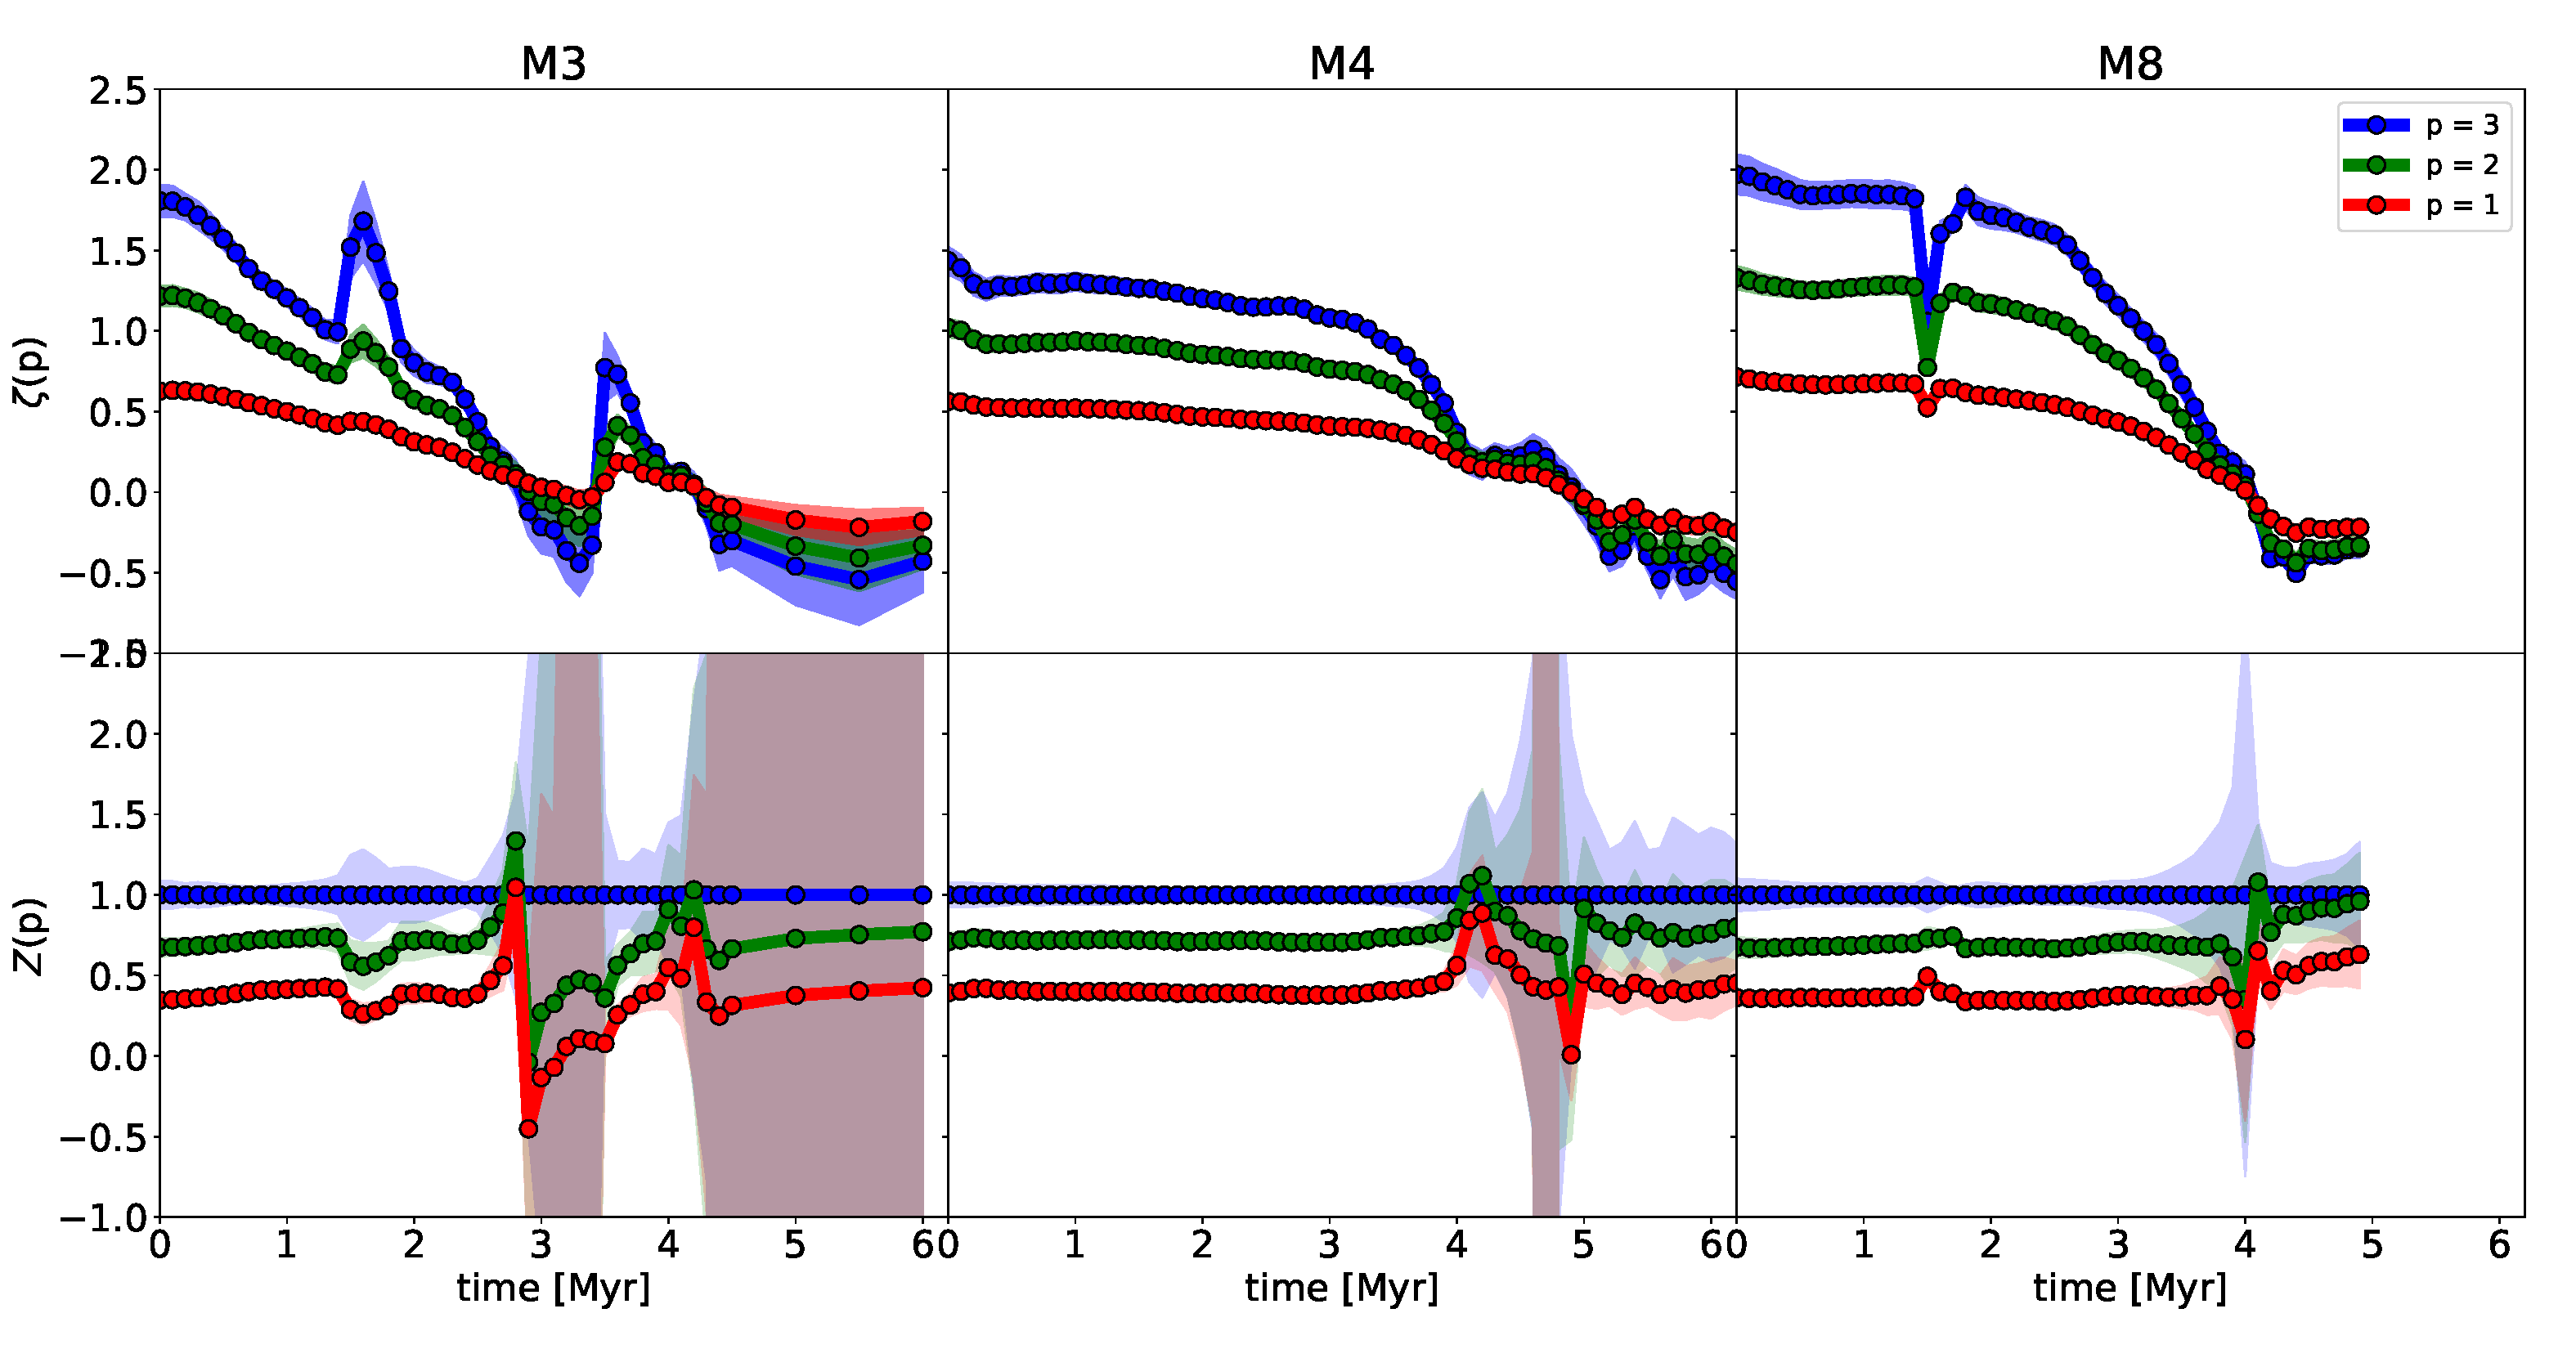
\includegraphics[width=0.9\textwidth]{error_vsf04_zeta_z.pdf}
    \caption{
        Data presented in Fig.~\ref{pic:results:zeta_all}a, with
        shaded areas behind the data representing the error ranges of the computed $\zeta$ (\textit{top}) and $Z$ (\textit{bottom}).  
%mm
    \mm{[left axis labels are clipped.]}
    }
    \label{pic:appFitting:error_vsfhr04_zeta_z}
\end{figure*}


\textbf{
%mm From \texttt{curve\_fit} we also obtain 
     The fit also provides    
the $\chi^2$ errors for the measured values of $\zeta$. 
    In Fig.~\ref{pic:appFitting:error_vsfhr04_zeta_z} we show a reduced version of Fig.~\ref{pic:results:zeta_all}(a), where
    we only plot the time evolution of $\zeta$ for all three clouds, along with
%mm    Additionally, we added 
shades of the same colours of the respective lines that represent the errors.
%mm areas as derived by \texttt{curve\_fit}.
    We see that the relative errors, $\Delta \zeta / \zeta$ mostly remain within a range of 5--12\%. 
%mm [rewrite to make meaning clearer]
    \mm{[not sure what this next means]}
    Only when $\zeta$ becomes very negative do the errors increase as it is harder to unify the fall in $S_\mathrm{p}$ with larger $\ell$ with the requirement that $S_\mathrm{p} (\ell=0)=0$ (as no relative velocity can be measured within one zone).
}

\textbf{
    The errors of $Z$ are computed by Gaussian error propagation
}
\begin{align}\Delta Z(p) &= \sqrt{ \left( \frac{\partial Z(p)}{\partial \zeta(p)} \cdot \Delta\zeta(p) \right)^2 + \left( \frac{\partial Z(p)}{\partial \zeta(3)} \cdot \Delta\zeta(3) \right)^2 } \\
        &= \sqrt{ \left( \frac{\Delta\zeta(p)}{\zeta(3)} \right)^2 + \left( \frac{ \zeta(p) \cdot \Delta\zeta(3)}{\zeta(3)^2} \right)^2 }.
        \label{equ:appFitting:z_error}
\end{align}
\textbf{
    \noindent In general, the relative errors of $Z$ are, as well, around 10\%, though
     we do see exceptions with very large errors. 
    The reason for these is that at these times $\zeta$(3) approaches zero, causing Eq.~(\ref{equ:appFitting:z_error}) to diverge.
}



\endinput
